\documentclass[
	12pt, % Font size
	a4paper, % Paper size
	oneside, % One-sided document
]{report}

% Set the PDF version for LuaTeX
\usepackage{luacode}
\begin{luacode}
  pdf.setminorversion(6)
\end{luacode}

% Packages
\usepackage[english]{babel} % Set document language
\usepackage{pdfpages} % Include PDF files
\usepackage[utf8]{inputenc} % UTF-8 encoding (for umlauts etc.)
\usepackage[T1]{fontenc} % correct hyphenation
\usepackage{csquotes} % correct quotation marks
\usepackage{lmodern} % Computer Modern fonts
\usepackage{microtype} % better typesetting results (avoids underfull / overfull hboxes)
\usepackage{graphicx} % adding graphics
\usepackage{units} % typesetting units, e.g. \unit[10]{MB} and \unitfrac[100]{Mbit}{s}
\usepackage{booktabs} % publication quality tables
\usepackage{titlesec} % Customize chapter and section headings
\usepackage{setspace} % Set line spacing
\usepackage{geometry} % Set page margins
\usepackage{subcaption}
\usepackage{float}
\usepackage[
	backend=bibtex,
	style=numeric-comp,
	maxcitenames=2,
	natbib=true,
	sorting=none
]{biblatex} % Bibliography

% Bibliography
\addbibresource{literature.bib}

% Title page
\title{Title of Your Thesis}
\author{Til Mohr}
\date{\today}

% Document
\begin{document}

% Title page
\maketitle

% Eidesstattliche Versicherung
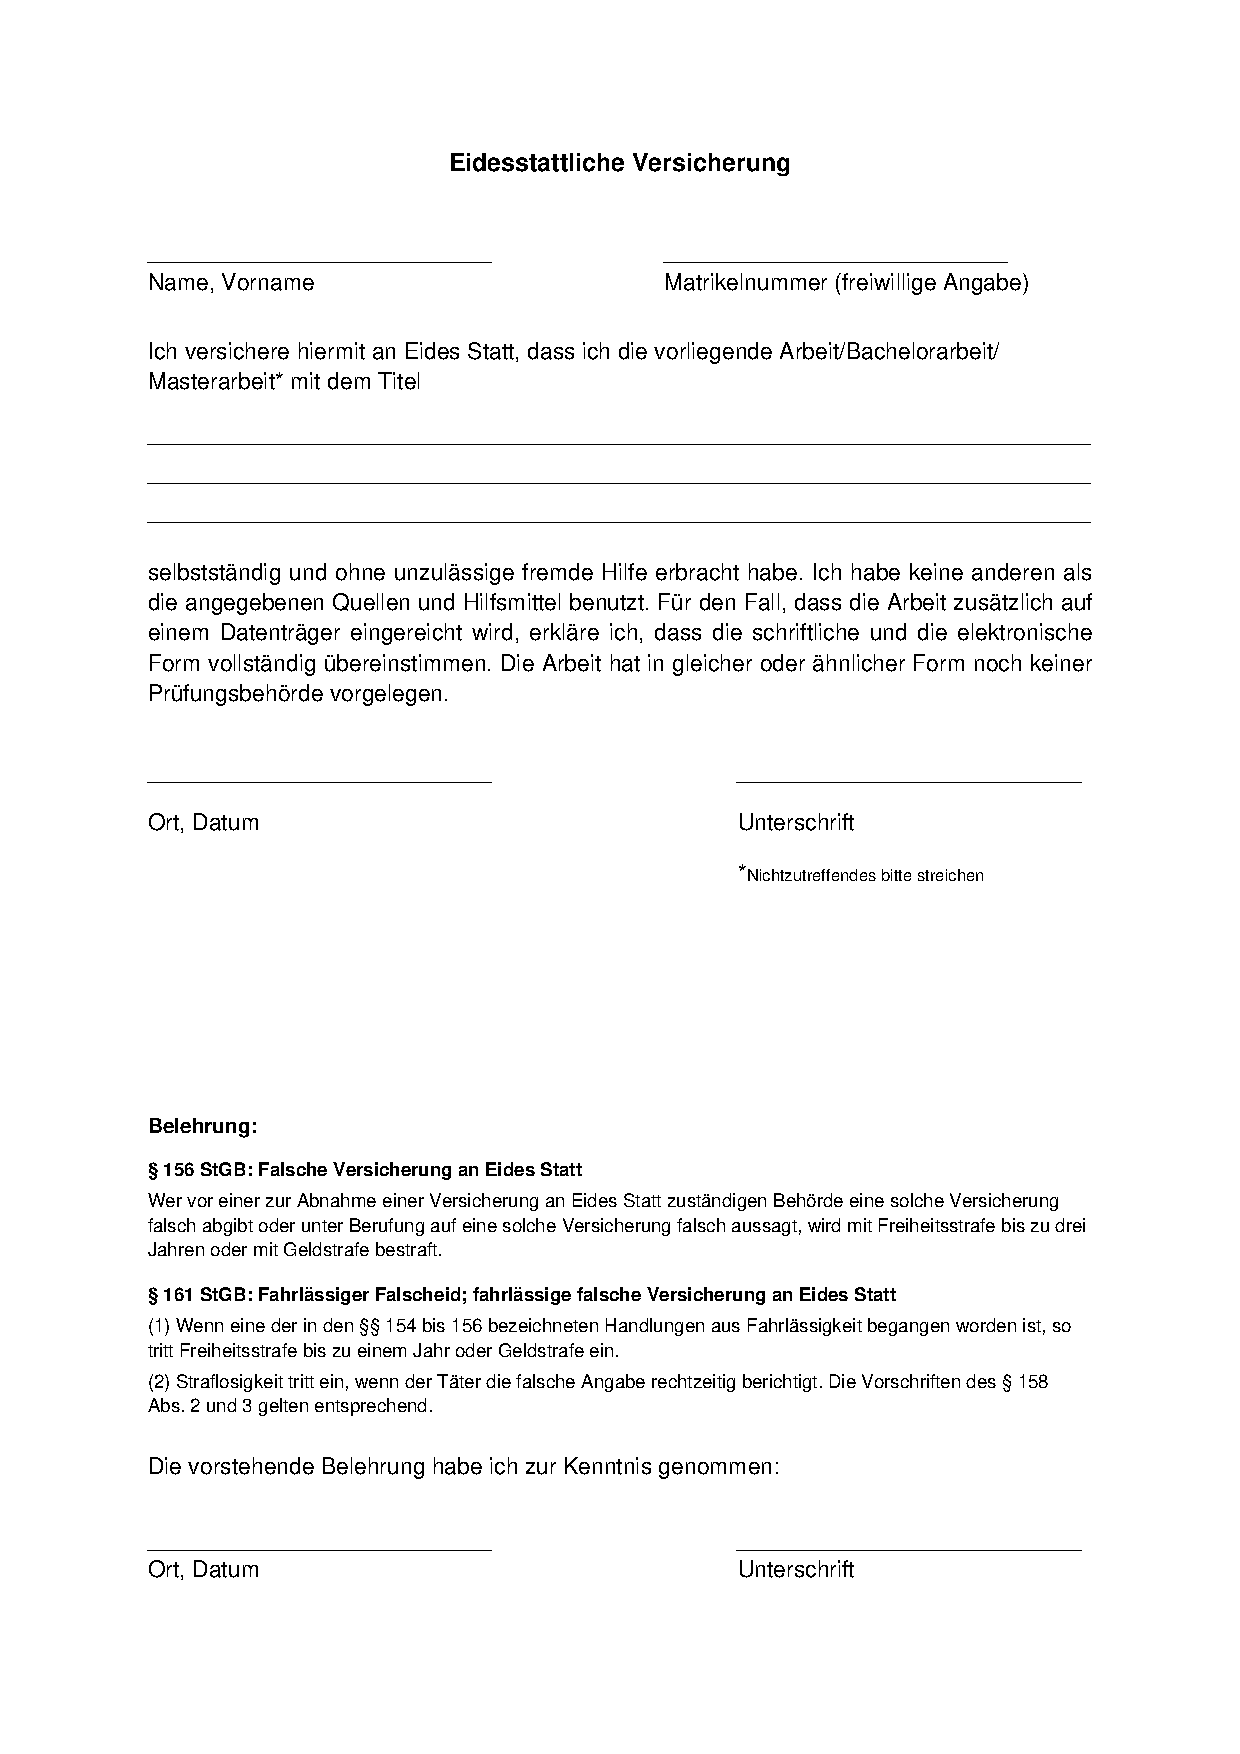
\includepdf{Formular_Eidesstattliche_Versicherung.pdf}

% Abstract
\begin{abstract}
This is the abstract of your thesis.
\end{abstract}

% Table of contents
\tableofcontents

% Chapters
\chapter{Introduction}
The development of efficient algorithms for solving large-scale mixed-integer programming (\MIP{}) problems has been a central focus of operations research for decades. Column generation, a powerful technique for solving large-scale linear programs, has been extended to integer programs through the branch-and-price algorithm. The effectiveness of branch-and-price relies heavily on the branching strategies employed and the ability to integrate various constraints into the reformulated problem during column generation.

In this thesis, we explore advanced branching rules and constraints within the context of the branch-and-price framework, particularly focusing on the implementation and evaluation of the component bound branching rule. This rule, as proposed by Desrosiers et al. \cite{thebook}, offers a simpler alternative to Vanderbeck's generic branching scheme \cite{vanderbeck2011branching} for branching on so-called component bound sequences \cite{vanderbeck1996exact}. As both branching rules operate entirely within the reformulated problem, integrating them into a branch-and-price framework requires careful consideration of the underlying mathematical structure and the implementation details.

The foundational concepts of polyhedron representation and the primal simplex algorithm are introduced in Chapter \ref{ch:preliminaries}, providing the mathematical and algorithmic background necessary for understanding the core methods discussed later. In Chapter \ref{ch:cg_bp}, we delve into the specifics of column generation and branch-and-price, detailing the algorithms and their implementation, including the Dantzig-Wolfe reformulation, which serves as the basis for the decomposition approach used in branch-and-price.

Chapter \ref{ch:tools} provides a brief overview of the \SCIP{} Optimization Suite, with a particular focus on the \GCG{} solver, which forms the foundation for the implementation work carried out in this thesis. In Chapter \ref{ch:cmpbnd}, we present the component bound branching rule in detail, including its separation procedure and a theoretical comparison to Vanderbeck's generic branching scheme.

One of the major contributions of this thesis is the introduction of a new interface within \GCG{} for handling constraints that exist solely within the master problem, termed \textbf{generic mastercuts}. These constraints, which do not have a direct counterpart in the original problem, require special handling within the solver, particularly with respect to synchronizing master variables across the search tree and applying dual value stabilization. Chapter \ref{ch:gm} begins by presenting the conceptual framework and definition of generic mastercuts, followed by an elaboration on the synchronization mechanisms and the application of dual value stabilization for these constraints, highlighting the technical innovations introduced in this thesis.

Chapter \ref{ch:implementation} focuses on the implementation aspects, detailing how the generic mastercut interface was integrated into \GCG{}, and how it supports the component bound branching rule.

The effectiveness of the component bound branching rule and the generic mastercut interface is rigorously evaluated in Chapter \ref{ch:evaluation}. We compare different separation heuristics and analyze the impact of dual value stabilization on the performance of the branching rule. Additionally, a detailed comparison with Vanderbeck's generic branching scheme provides insights into the conditions under which the component bound branching rule may offer advantages.

\chapter{Conclusion}

% References
\begin{thebibliography}{9}
\bibitem{ref1} Author. \textit{Title of the Reference}. Publisher, Year.
\end{thebibliography}

\end{document}

% End of document
\end{document}